\documentclass{proseminar}

\let\i\undefined
\let\c\undefined
\let\b\undefined
\newcommand{\i}[1]{\emph{#1}}
\newcommand{\c}[1]{\texttt{#1}}
\newcommand{\b}[1]{\textbf{#1}}
\begin{document}

\conferenceinfo{Albert-Ludwigs Universit\"at Freiburg\\Technische Fakult\"at, Institut f\"ur Informatik\\Lehrstuhl f\"ur Datenbanken \& Informationssysteme}{}

\title{Trust and Privacy in Social Media \\
\huge Content oriented trust}

\numberofauthors{1} 
\author{
Tim Schmiedl\\
\email{tim.schmiedl@neptun.uni-freiburg.de}
}

\maketitle

\section{Introduction}
Over the last couple of years microblogging became a well-established paradigm for interaction in online social networks.
Especially the success of Twitter let to an increase of huge amount of real-time informations on the internet. It lets user post short messages which are shown immediately for their followers. This concept was of course quickly adapted by news agencies, product pages and many other. So nowadays Twitter displays a wide variety of content. Most tweets correspond to the following categories; conversation items, which are just valuable to user and its immediate circle of friends, or information or news items, which could be interesting for a broader community.

%* mobile internet devices 
%* propagating news and information about developing events 

% =========================

\subsection*{Current Situation}
Twitter was well known to display tweets in reverse chronical order displaying what is happening right now on the very top of the news feed. 
The microblogging company itself tried to experiment in some ways to show the information in different ways, one is to show popular tweets on top regardless of the posting time.
This decision was often criticized as it often shows for the user unrelevant information or advertisement. This position of popular tweet was also often the target of internet trolls or spammers trying pollute the news feed of many users.

As microblogging has become more and more popular it was shown that beside chatting about events on a day-to-day basis it can be in particularly helpful during emergency and/or crisis situations.
Twitter provide real-time information from the actual location where the crisis is unfolding. This information often spreads faster and to a wider audience than what traditional news media sources can achieve.


% =========================

\subsection*{Problems}
Twitters ranking method of displaying popular tweets as not taken into account content relevance or the twitter account.
This lets a large amount of pointless tweets may flood the relevant tweets of the users news feed. It also allows for more potential for spam to spead, as it is not filtered in this ranking method.

As a result of the big variety of content and different kinds of users it is very difficult to differentiate between news related topics and chat between user. Finding tweets which have valuable information outside its immediate circle of friends or follower is often not easy as there is no distinction between different kind of messages. 


% =========================

\subsection*{Goals of the Papers}
The primary element of this report are the two papers P1 and P2.

P2\cite{P2} proposes a method to rank tweets based on their content relevance to a given query. They use different set of features to find out weather a tweet is interesting for a user. Their \i{learning to rank} algorithm considers content relevance as well as account authority and twitter-specific features to rank tweets. In their evaluation they find out that especially if a URL is present in the tweet improves the relevance as well as that just the number of followers to an account doesn't directly correlates to bigger relevances of tweets from that author.

In P1\cite{P1} the authors had a the main focus on the credibility of time-sensitive information, in particular on current news events. In a previous step they also try to automatically assess the newsworthiness of a discussion topic. This is to differentiate between the chatter and news related messages circulating on twitter in unsorted way. Both newsworthiness and credibility play an equally important role in this paper.

% =========================
% =========================
% =========================


\section{Twitter Case Study}
P1 presents a case study about information propagation during a crisis event on twitter. The authors describe differences in how a sample of confirmed news and false rumors propagate in the aftermath of the 2010 Earthquake in Chile. This case study provides some valuable insight into credibility characteristics in microblogging.


\paragraph{Event characterization}
On Saturday, February 27, 2010 at 03:34 local time an earthquake occurred just off the coast of the Maule region of Chile. It reached a magnitude of 8.8 on the Richter scale and lasted for 90 seconds and is therefor one of the ten strongest earthquakes ever recorded in history. Minutes after the earthquake, a
tsunami reached the Chilean shores. Nearly 560 people died and more than two million people were directly affected by the crisis.

In the hours and days after this earthquake, Twitter was used to post time-critical information about tsunami alerts, missing people, deceased people, available services, interrupted services, road conditions, functioning gas stations, among other emerging topics related to the catastrophe. After the earthquake, bloggers published first-hand accounts on how they used twitter during the emergency\cite{p1previouswork}.


\paragraph{Reactions and Rumors}
The earthquake reached the level of trending topic in Twitter a few hours after the event. The authors of P1 collected public tweets concerning the topic by searching for specific keywords and hashtags as well as time zones (time zone of Santiago GMT-04:00). In total they collected over 4.700.000 tweets from over 700.000 different users  which registered an average of 1,018 followers and 227 followers at the time of the earthquake. 
Figure Figure \ref{fig:p1propgation} shows that tweets with the term "earthquake" are propagated through the social network.

\begin{figure}[h]
\centering
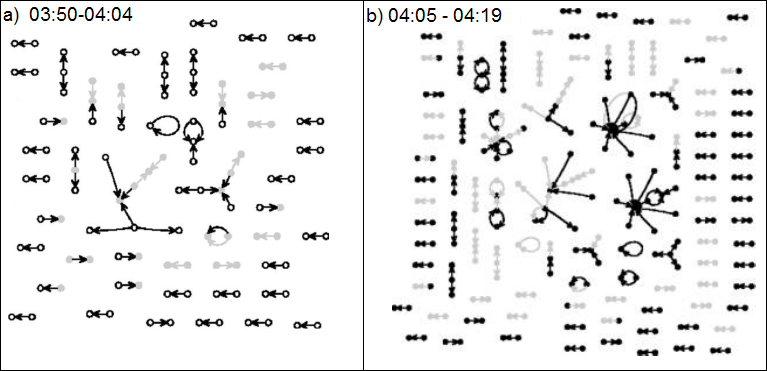
\epsfig{file=img/p1_propgation.png, width=0.45\textwidth}
\caption{Trend propagation}
\label{fig:p1propgation}
\end{figure}

\begin{figure}[h]
\centering
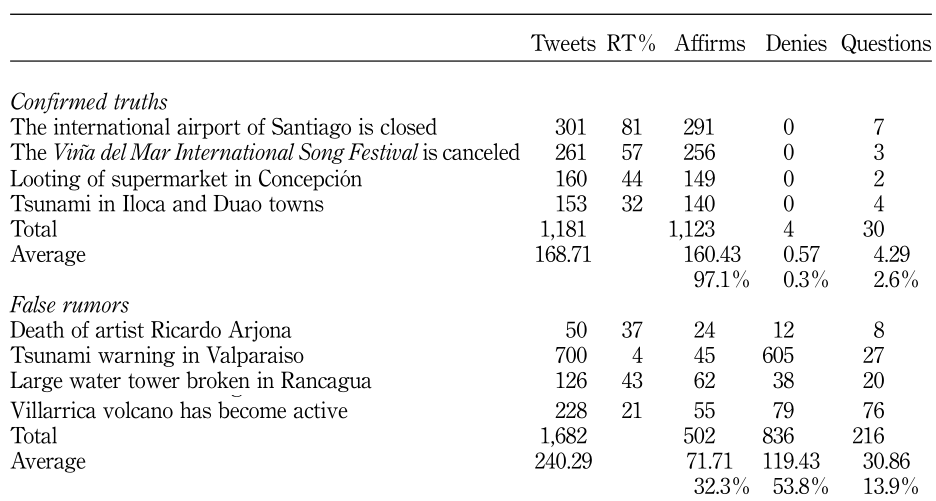
\epsfig{file=img/p1_rumors.png, width=0.45\textwidth}
\caption{Number of "affirms" and "Denies" of truths and false rumors}
\label{fig:p1rumors}
\end{figure}



% =========================
% =========================
% =========================

\section{Proposed Method: Ranking of \\Tweets}
This section describes the method of ranking of tweets introduced in P2. 
Their \textit{learning to Rank} method is a data-driven approach to assign a score to tweet. 
For training the ranking model the RankSVM\cite{ranksvm} algorithm is used.

Figure \ref{fig:p2overview} shows the the paradigm of the method and the separation of the training and test corpus.

\begin{figure}[h]
\centering
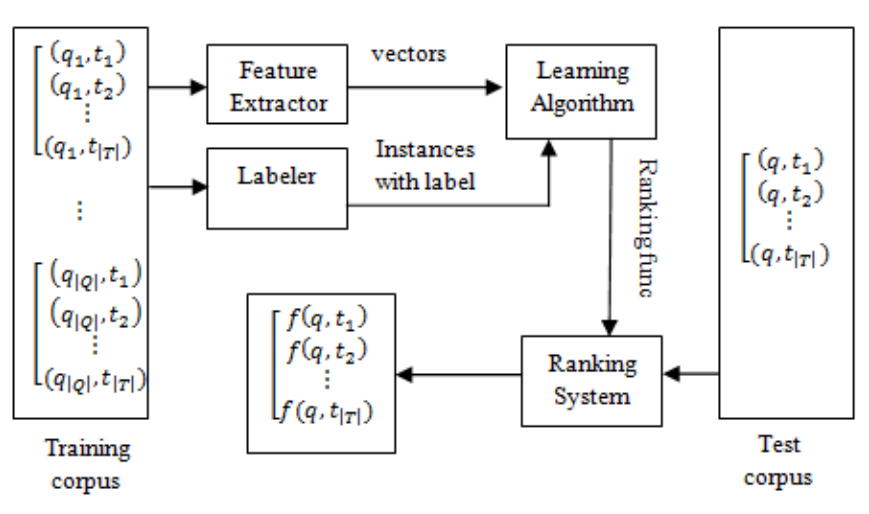
\epsfig{file=img/p2_overview.png, width=0.45\textwidth}
\caption{General Paradigm of Learning for Tweets Ranking}
\label{fig:p2overview}
\end{figure}

The learning to rank system used three types of features: Content relevance features, Twitter specific features and Account authority features

\subsubsection*{Content relevance features}
The content relevance features refer to those features which describe the content relevance between queries and tweets.
P1 uses three different types of content relevance:

\begin{itemize}
\item \b{Okapi BM25}\cite{okapi} score measures the relevance between query and tweet. It considers the length of a tweet, the average length of tweets and the Inverse Document Frequency.
\item \b{Similarity of contents} how many tweets of the query are similar in content with the current tweet. To accomplish that the cosine similarity between every pair of tweets is computed.
\item \b{Length} is simply measured by the number of words that a tweet contains.
\end{itemize}


\subsubsection*{Twitter Specific Features}
As the proposed method is tested on twitter it also relies on some of the Tweet-specific features. 

\begin{itemize}
\item \b{URL and URL Count} Tweets can contains one ore more URLs in the composed message. The feature URL hereby is a binary feature indicating with 1 if there is a URL present, whereas the URL Count estimates how often a particular URL is found in the tweet corpus.
\item \b{Retweet Count} Twitter users can forward a tweet to his or her followers with or without modification on the forwarded tweets. In this feature Retweet count is defined as the number of times a tweet is retweeted.
\item \b{Hash Tag Score} Hashtags are a type of label or metadata tag microblogging services, especially on twitter, which makes it easier for users to find messages with a specific theme or content. For this feature hashtags are collected from all tweets and sorted in descending order. The feature score correlates with the frequency of hashtags in the tweet with the most frequent hashtags.
\item \b{Reply} This is a binary feature. It is 1 when the tweet is a reply and 0 otherwise.
\item \b{Words out of vocabulary} This feature is used to roughly approximate the language quality of tweets. The vocabulary is defined by the words of a dictionary with 0.5 million entries.

\end{itemize}

\subsubsection*{Account Authority Features}
There are three important relations between users in Twitter: follow, retweet, and mention. 
In general user are seen as more authoritative if they have more followers, been mentioned in more tweets, listed in more lists and retweeted by more important users.

The main assumption here is that tweets are more likely to be informative if posted or retweeted by authoritative user.

To compute the authority of the user, P2 uses four different scores:
\begin{itemize}
\item \b{Follower score} number of followers a user has.
\item \b{Mention score} number of times a user is referred to in tweets.
\item \b{List score} number of lists a user appears in
\item \b{Popularity score} computed by PageRank algorithm (Page et al., 1999)\cite{pagerank} based on retweet relations.
\end{itemize}

\subsection*{Evaluation}
\subsubsection*{Dataset}
To test the proposed method the authors of P2 analyzed hot searches on CrowsEye within a week and collected the messages of 20 of the most frequent searched query terms. The terms included 5 persons 5 persons, 5 locations, 5 products and 5 movie names. 
In total there were 159,298 tweets captured in the time between Mach 25, 2010 and April 2, 2010.

For the generation of a test dataset 500 tweets of each query was labeled by a human editor. The evaluators could apply four judgments grades on the tweets depending on their relevance to the search query. 
The distribution of the grades were as follows: Excellent 20.9 \% ; Good 10.9\%; Fair 16.9\%; Bad 51.3\%.


\subsubsection*{Results}
For comparison the authors of P2 used the Normalized Discount Cumulative Gain (NDCG) metric, which is common to measure the quality of rankings.

The ranking model, RankSVM, was tested on different types of feature subsets. The main types were 
The main types of feature subsets proposed by the the authors are chronological order, account authority, and content relevance. Figure \ref{fig:ranking} shows the result of these rankings individually and also the combined or full set of features which is denoted as RankSVM\_Full.

\begin{figure}[h]
\centering
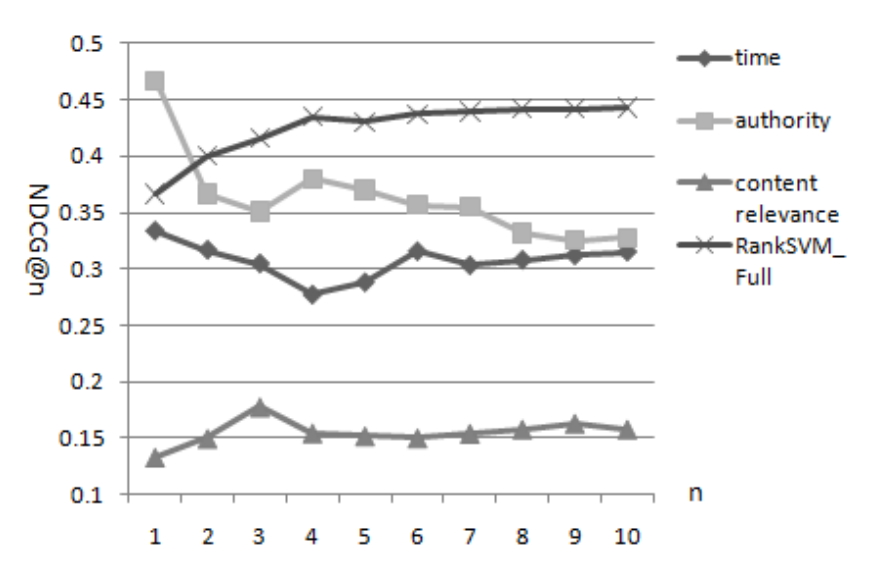
\epsfig{file=img/p2_results.png, width=0.45\textwidth}
\caption{Performance of Four Ranking Methods}
\label{fig:ranking}
\end{figure}

It is clearly visible that content relevance is the worst type, which should not come as a surprise as it is essential a re-ranking of the results of the Twitter search. It is also shown that account authority is useful for ranking tweet relevance, as it outperforms ranking through chronological order and compete with the model trained with all the features.

In the next part of the evaluation the authors of P2 tried to find out which feature as well as which combination of features showed the best results.
To complete this evaluation a greedy feature selection method was used to find the best feature conjunction which outperforms RankSVM\_full. The best feature conjunction was found to be composed of the features URL, Sum\_mention, First\_List, Length, and Important\_follower and denoted as RankSVM\_Best. It outperforms RankSVM\_full by about 15,3 \% at NDCG@10.

In the final evaluation it was tested which of the six features in particular had the most significant effect on RankSVM\_Best. Here the authors of P2 evaluate the importance of each feature by the decrement of performance when removing the feature measured from RankSVM\_Best. 
Figure \ref{fig:p2_resultFeature} shows that only the feature URL has a significant effect.

\begin{figure}[h]
\centering
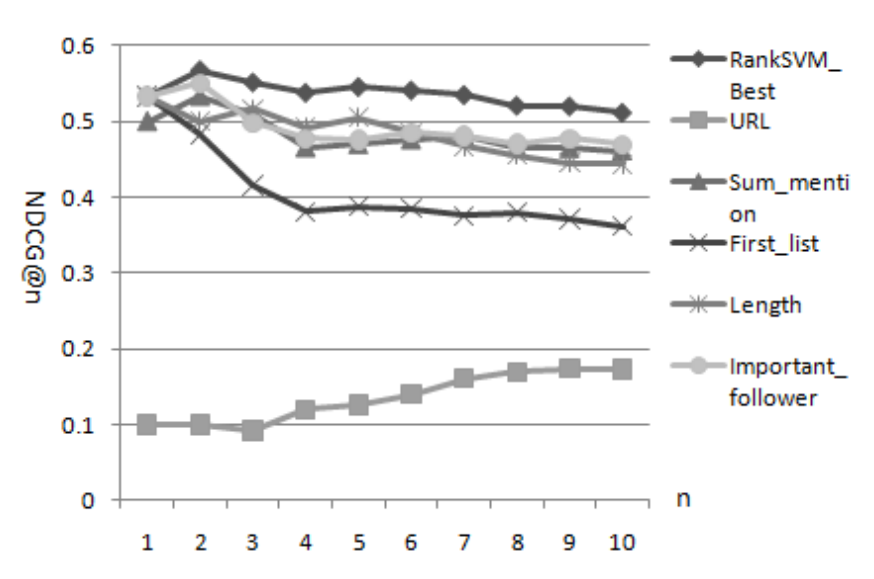
\epsfig{file=img/p2_results_features.png, width=0.45\textwidth}
\caption{Importance of Each Feature}
\label{fig:p2_resultFeature}
\end{figure}


% =========================
% =========================
% =========================

\section{Proposed Method: Prediction\\ Model for Tweets}
P1 proposes a method to automatically distinguish between different types of messages in time-sensitive social media like on Twitter.
The paper follows a supervised learning approach for the task of automatic classification of credible news events. A first classifier decides if an information cascade corresponds to a newsworthy event. Then a second classifier decides if this cascade can be considered credible or not.

% In Section 4 we present the process of creating a labeled data set of newsworthy events for credibility assessment. This procedure is performed using crowdsourcing tools

\subsection{Retrieving and Labeling of Data}
It should be noted that the work of P1 is based on previous works and is an information cascade, which is composed of all of the messages which usually accompany newsworthy events. This means that only aggregated values of a topic are computed and compared, not on user or message level.

For the collection of data on Twitter they used Twitter Monitor\cite{twittermonitor}, which detects sharp increases (bursts) in the frequency of sets of keywords found in messages. It provides a keyword-based query to filter messages to generate a subset of messages who caused the event detector to trigger.
During their 2 month of monitoring twitter, they collected, after some rough filtering, more than 2.500 topics with ofter 1.873.000 messages in total.

\subsubsection*{Newsworthiness}
The first step was to  separate newsworthy topics amongst all the collected data. The task hereby was to distinguish between conversation or chat messages which have little importance outside a reduced circle of friends and newsworthy topics with the potential to be of interest to a broader set of people.

For the labeling process the authors of P1 used human editors and explored the crowdsourcing tool Mechanical Turk for the characterization of topics.
The human editors were asked if most of the messages were spreading news about a specific event (labeled as class NEWS) or mostly comments or conversation (labeld as class CHAT). To  reduce the effect of click spammers in the evaluation system the evaluators were asked to provide a short summary sentence of the topic.

In this process P1 selected randomly 383 topics with 221.279 in total. From this 383 topics 34.9 percent were labeled as CHAT, 29.5 percent as NEWS and 35.6 percent remained as UNSURE.


\subsubsection*{Credibility}
After the classification according to newsworthiness the topics in the NEWS class, aka the newsworthy topics, should be rated in a credibility aspect.
This second round of manual label takes the output of the previous manual classification as well as data from the automatic classifier build using the manually labeled data as input. With the use of the automatic classifier P1 was able to expand the amount of newsworthy topics to 747 cases.

The topics consisting of many tweets were again presented to a human evaluator for judgment. Again they were asked via an Mechanical Turk interface to rate the topics according to for topics: "almost certainly true", "likely to be false", "almost certainly false" or "uncertain". To reduce the effect of spammers they were again asked to provide a short justification sentence. 

The result of the credibility classes were as follows:
\begin{itemize}
\item 306 cases were "almost certainly true", 41 percent
\item 237 cases were "likely to be false", 31.8 percent
\item only 65 cases were "almost certainly false", 8.6 percent
\item 139 cases were "uncertain", 18.6 percent
\end{itemize}

\subsection{Prediction Model for Tweets}
The main hypothesis of P1 is that the level of newsworthiness and credibility can be estimated automatically. To accomplish that task they build to different classifier. In the following two sections it is described which factors are useful to establish  information credibility and which features are most useful for automatic estimation of newsworthiness and credibility.

%We believe that there are several factors that can be observed in the social media platform itself that are useful to establish information credibility. These factors include:
%* 1. reactions and emotion, opions, negative/positive sentiments 
%* 2. certainty, question info or not?
%* 3. sources cited, URLs, popular domain
%* 4. propagation characteristics, which user, how many follower etc.

\subsubsection*{Automatic discovery of newsworthy topics}
To train the supervised classifiers to determine if a set of tweets describes a newsworthy event or not the labeled data of the supervised training phase is uesed. As a reminder the labels consider the three classes NEWS, CHAT, UNSURE. Preliminary evaluations showed a negative effect of the UNSURE label, therefore it was decided to remove instances with the UNSURE label completely form the training data set.

\paragraph{Learning scheme}
P1 tested different machine learning schemes to run on the data, they included Naive Bayes, Bayes Net, Logistic Regression, and Random Forest. The results of the comparison showed that Bayes Net was the best learning scheme in this scenario, although Random Forest performed almost equally well.

\paragraph{Feature subset}
After the testing of the different learning schemes P1 studied how different features  contribute in the prediction of newsworthy topics.
The following subsets were investigated:

\begin{itemize}
\item \b{Text-only subset} considers all the features of the message text. This includes for example the average length of the tweets,
sentiment-based features, features related to URLs or twitter-specific features like hashtags or user mentions. In total 20 different features are contained in this subset.
\item \b{User subset} considers all of the features which represent the social network of users. This includes metrics like number of friends or number of followers. This subset contains the seven features.
\item \b{Topic subset}  considers all of the topic features which include the fraction of tweets that contain one of these four elements (at topic level): most frequent URL, most frequent hashtag, most frequent user mention, and most frequent author
\item \b{Propagation subset} considers the propagation-based features plus the fraction of re-tweets and the total number of tweets. This subset contains the seven different features.
\end{itemize}

\begin{figure}[h]
\centering
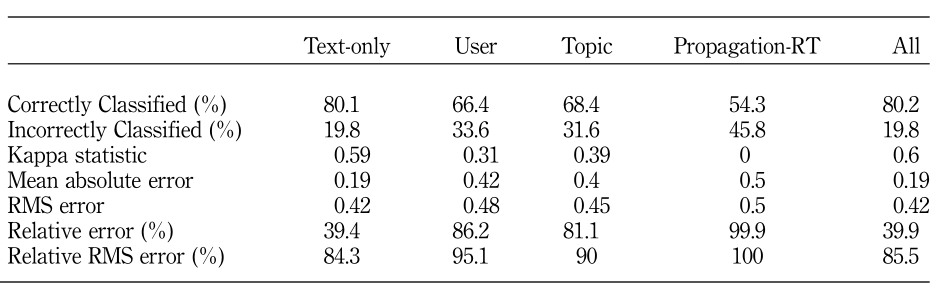
\epsfig{file=img/p1_table_feature_subset.png, width=0.45\textwidth}
\caption{Results for different feature subsets}
\end{figure}

\paragraph{Feature selection}
With the manually labeled test data P1 were able to compare the effects of different feature subsets on the test data. A small part of the results of this comparision is shown in Figure \ref{fig:boxNews}.

\begin{figure}[h]
\centering
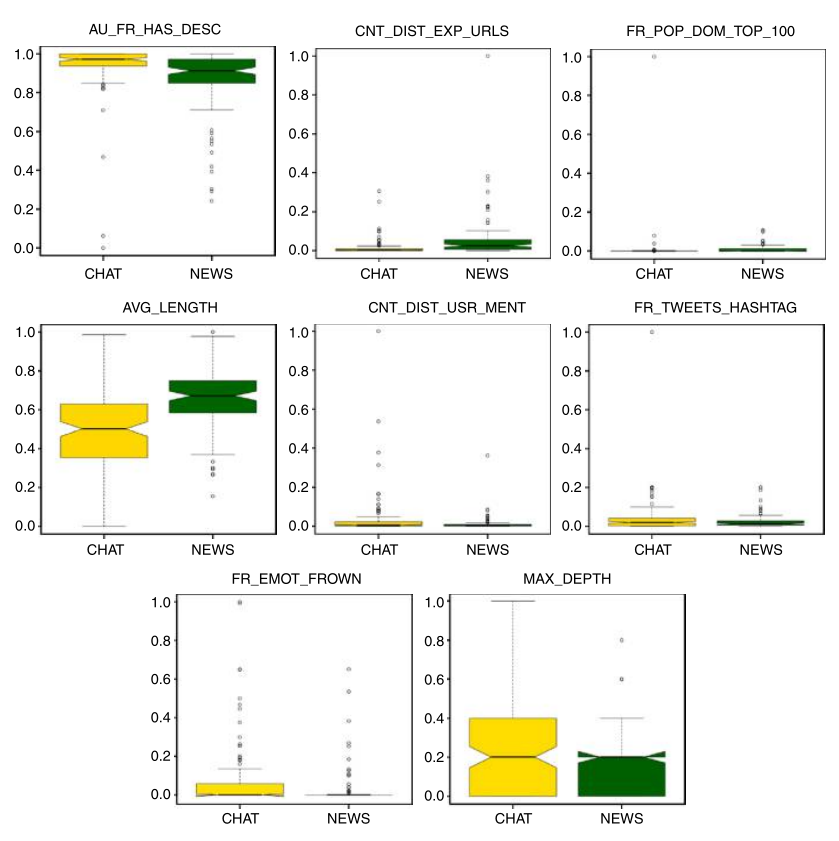
\epsfig{file=img/p1_box_news.png, width=0.45\textwidth}
\caption{Boxplots depiction the distribution of features best separating newsworthy and chat topics}
\label{fig:boxNews}
\end{figure}

The analysis shown in Figure \ref{fig:boxNews} shows eight different features and their effect on newsworthiness. It is shown that authors with a description in their profile are more likely to propagate chat. 
Topics which have longer tweets tend to be more related to news topics. Newsworthy topics also share more URLs which belong to the top-100 most popular domains but contains less frown emoticons than chat related topics, which might be quite intuitive.
Also, news topics tend to have less hashtags than chat, and contain more URLs in general.


\subsubsection*{Credibility prediction}
The task of the second classifier is to assign a credibility level (or score) to a topic deemed newsworthy by the previous classifier.

\paragraph{Data selection}
The manual labeling process introduced 4 types of classes concerning credibility of topics:  "almost certainly true"," likely to be false",  "almost certainly false" and "uncertain". To train the classifier this problem was reduced to a binary classification were topics with the almost certainly true label are assigned to a new class CREDIBLE and all others combined in the class NON-CREDIBLE.
In total there were 152 topic instances of class CREDIBLE and 136 in the class NON-CREDIBLE which correspond to a class balance of 47.2/52.8 percent. The topics consists of  165,312 tweets in total. 


\paragraph{Learning scheme}
Again there was a need for a learning scheme for the training of the classifier. Similar to the previous classifier different learning schemes were tested to check the performance on the credibility assesment. The results of the best schemes, Random forest, Logistic and Meta learning are pictured in Figure \ref{fig:schemeCredibility}.

\begin{figure}[h]
\centering
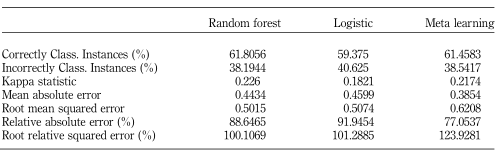
\epsfig{file=img/p1_scheme_credibility.png, width=0.45\textwidth}
\caption{Results of different lerning algorithms with respect credibility assessment}
\label{fig:schemeCredibility}
\end{figure}

As the results shows the predictability of the problem seems to be very difficult. Especially the misclassification of not-credible topics as credible is significant and the moderate kappa-statistic values indicate that improvements over a random predictor are limited.

\paragraph{Feature selection}
Analogous to the detection of newsworthiness the credibility classifier was tested on different features and feature subsets. Some of these features are shown with their corresponding boxplots in Figure \ref{fig:boxCredibility}:

\begin{itemize}
\item AVG\_STAT\_CNT, the average number of tweets posted by authors of the tweets in the topic in the past
\item FR\_SENT\_POS, the fraction of tweets having a positive sentiment
\item FR\_SENT\_NEG, the fraction of tweets having a negative sentiment
\item FR\_EMOT\_SMILE, the fraction of tweets containing a “smiling” emoticons
\item FR\_PRON\_FIRST, the fraction of tweets containing a first-person pronoun
\item FR\_PRON\_THIRD, the fraction of tweets containing a third-person pronoun
\item FR\_TWEETS\_URL, the fraction of tweets containing a URL
\item FR\_POP\_DOM\_TOP\_10000, the fraction of URLs pointing to a domain among the top 10,000 most visited ones
\item FR\_TWEETS\_QUEST\_EXCL\_MARK, the fraction of tweets containing a question or an exclamation mark
\end{itemize}


\begin{figure}[h]
\centering
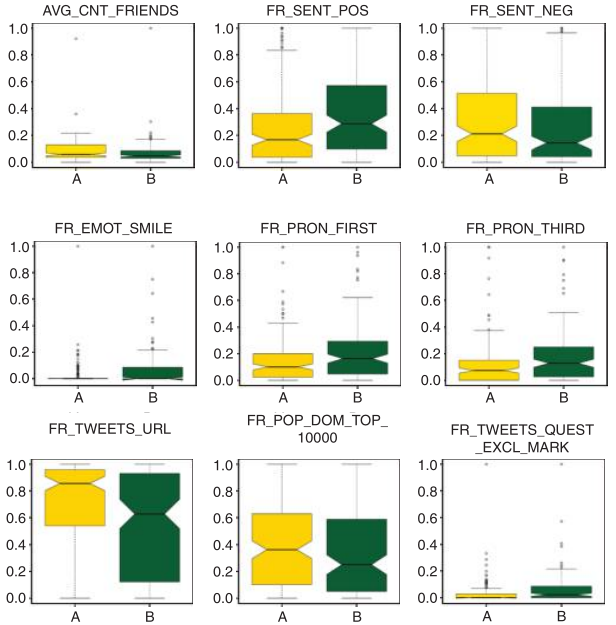
\epsfig{file=img/p1_box_credibility.png, width=0.45\textwidth}
\caption{Boxplots dipicting distribution of different features, A represents credible, B represents non-credible topics}
\label{fig:boxCredibility}
\end{figure}

The analysis of the feature selection showed that tweets with more URLs and in particular URLs which are included on the top-10.000 most visited domains belongs to credible topics. 
Regarding polarity, non-credible tweets tend to concentrate more positive polarity scores, as opposite to credible tweets, which tend to express negative feelings.
In contrast to credible topics, authors of tweets classified as non-credible concentrate question and exclamation marks, frequently use first and third-person pronouns and include much more emoticons.


% =========================
% =========================
% =========================

\section{Comparision of the papers}
Both papers, P1 and P2, study the information propagated via microblogging especially on Twitter. They try to get more that just the text information on messages or tweets by considering additional features like the authors or the propagation of tweets.

\paragraph{Goals of the papers}
Both paper try to get additional information on tweets and compositions of tweets by looking at meta-information and analysis of different features.
P2 tries to find relevant tweets to a given topic. For that the authors proposed a ranking model which assigns a score for relevance for each tweet given a topic.
P1 has two different goals, first they try to find topics (compositions of many tweets) which are newsworthy in an automatic manner to then present to a second classifier, which rates the credibility of the newsworthy topics.

\paragraph{Similarities and differences}
As the topic of both papers is in the same area, they explore some similar techniques and consider similar features. Both papers classify the types of features in a similar way; text related features like length of messages as well as the presents of URLs, user features like the number of friends, but also twitter-specific features like hashtags or user mentions.

Apart from the slightly different goals there are also some differences in the approach of the authors of P1 and P2. P1 doesn't consider single tweets as own entities but aggregate many tweets into a unit and study the resulting information cascades. The classifier built by the authors of P1 use binary classification (Newsworthy vs Chat or Credible vs Non-Credibile).
The smallest unit in P2 are the text-messages itself, they are not classified in two classes but are rated in a continuously manner for their relevance given a topic.

\paragraph{Results}
Both papers did extensive evaluation of their methods, they come to the conclusion that different features have more or less influence on the relevance, respectively newsworthiness and credibility. Especially the presents of URLs seem to increase the quality of a tweet, it seems that the constriction of 140 characters in a tweet limits the expression of interesting information quite significantly. Also the effect of longer messages in general suggest the intuitive notion that longer text contain more information than shorter text.

% author feature: not so intuitiv but work also

\paragraph{Paper review}
Both paper collect messages from twitter not directly from the news stream but through different tools. P1 uses Twitter Monitor whereas P2 uses query searches form CrowdEye.
That is an issue because the tools already uses different query and search filters to find and aggregate tweets for a given search query. As a result the messages obtained through the tools are already pre-filtered in a way which might influence the results of the presented methods.
This is very apparent in P2 and the content-relevance feature which shows significant worse results then other types of features. 

P1 uses binary classification for the assessment of newsworthiness and credibility. As the author already mention in their evaluation chapter, this does often not reflect real life scenarios. Often it is hard even for a human to decide weather a topic is newsworthy or not as well as if certain information is totally credible or not.



















% =========================
% =========================
% =========================



\bibliographystyle{abbrv}
\bibliography{bibliography} 

\balancecolumns

\end{document}
